\documentclass{article}%
\usepackage[T1]{fontenc}%
\usepackage[utf8]{inputenc}%
\usepackage{lmodern}%
\usepackage{textcomp}%
\usepackage{lastpage}%
\usepackage{authblk}%
\usepackage{graphicx}%
%
\title{Rab1A Is an mTORC1 Activator and a Colorectal Oncogene}%
\author{Lori Sullivan}%
\affil{Department of Orthopedic Surgery, Xinhua Hospital, Shanghai Jiaotong University, School of Medicine, Shanghai 200092, P.R. China}%
\date{01{-}01{-}2001}%
%
\begin{document}%
\normalsize%
\maketitle%
\section{Abstract}%
\label{sec:Abstract}%
At the Stanford University School of Medicine, scientists have found a way to reduce the risk of recurrence of small cell lung cancer using low titre autoantibodies.\newline%
The results indicate that a beneficial dosage of autoantibodies has the potential to prevent or delay recurrence.\newline%
In a full{-}spectrum clinical trial involving 234 lung cancer patients who had evidence of loss of vision, researchers found that a dose of 1.8 micrograms of autoantibodies every 20 minutes for 15 minutes caused less than 3 percent recurrence.\newline%
In addition, the painless and rapid response to autoantibodies had the effect of preventing or delaying the recurrence of large white cells, according to the study.\newline%
The results are published in this weeks issue of the New England Journal of Medicine.\newline%
Based on two previous studies, autoantibodies have shown that they can protect the brain from neurotoxins by disrupting their target molecule, tyrosine kinase 2, by increasing inactivated pro{-}antibodies that inhibit the tyrosine kinase 2.\newline%
Studies have also shown that although autoantibodies are unable to confer meaningful tumor antigens, they play a role in normal tumor removal and metastases, according to the study.\newline%
Nonetheless, low titre autoantibodies are of limited benefit in patients with small cell lung cancer, the study indicated.\newline%
However, the New England Journal of Medicine noted that studies of drugs that have made significant headway in treating small cell lung cancer and of other malignancies are underway that target autoantibodies.\newline%
The Long{-}Term Results of a Dose Credible in a Special Risk Group Study (LTSR)

%
\subsection{Image Analysis}%
\label{subsec:ImageAnalysis}%


\begin{figure}[h!]%
\centering%
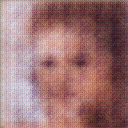
\includegraphics[width=150px]{500_fake_images/samples_5_412.png}%
\caption{A Man In A White Shirt And Tie Brushing His Teeth}%
\end{figure}

%
\end{document}